\documentclass[a4paper]{article}
\title{HHS - Håndværkernes HåndteringsSystem}
\author{
    Dam, Rasmus Kjær\\
    \texttt{rasm179f@edu.eal.dk}
    \and
    Rasmussen, Anders Fredensborg\\
    \texttt{ande714b@edu.eal.dk}
    \and
    Sandbøl, Kaare Veggerby\\
    \texttt{kaar1498@edu.eal.dk}
    \and
    Thomsen, Johannes Ehlers Nyholm\\
    \texttt{joha321j@edu.eal.dk}
    }
% Danish symbols.
\usepackage[utf8]{inputenc}
\usepackage[danish]{babel}
\usepackage[T1]{fontenc}

%4th layer of nesting
\usepackage{titlesec}
\setcounter{secnumdepth}{4}
\titleformat{\paragraph}{\normalfont\normalsize\bfseries}{\theparagraph}{1em}{}
\titlespacing*{\paragraph}
{0pt}{3.25ex plus 1ex minus .2ex}{1.5ex plus .2ex}

%Book tables
\usepackage{booktabs}

%Linebreak after subparagraph
\titleformat{\subparagraph}
    {\normalfont\normalsize\bfseries}{\thesubparagraph}{1em}{}
\titlespacing*{\subparagraph}{\parindent}{3.25ex plus 1ex minus .2ex}{.75ex plus .1ex}

%Images
\usepackage{float}
\usepackage{graphicx}
\graphicspath{ {./Images/} }
\usepackage{rotating} %Rotate pictures

%Links and clickable ToC
\usepackage{hyperref}

% Bibliography.
% \usepackage[options]{natbib}

% Page number
\usepackage{lastpage}
\usepackage{fancyhdr}
\pagestyle{fancy}
\fancyhf{}
%\fancyhead[L]{Top Left}
%\fancyhead[C]{Top Center}
%\fancyhead[R]{Top Right}
\renewcommand{\headrulewidth}{0.4pt}
%\fancyfoot[L]{Bottom Left}
\fancyfoot[C]{\thepage}
%\fancyfoot[R]{Bottom Right}
\renewcommand{\footrulewidth}{0.4pt}
\cfoot{\thepage\ of \pageref{LastPage}}

%longtable
\usepackage{longtable}
\usepackage{booktabs}

\usepackage{verbatim}

% Code
\usepackage{listings}
\usepackage{color}

\definecolor{dkgreen}{rgb}{0,0.6,0}
\definecolor{gray}{rgb}{0.5,0.5,0.5}
\definecolor{mauve}{rgb}{0.58,0,0.82}

\lstset{frame=tb,
  language=csh,
  aboveskip=3mm,
  belowskip=3mm,
  showstringspaces=false,
  columns=flexible,
  basicstyle={\small\ttfamily},
  numbers=none,
  numberstyle=\tiny\color{gray},
  keywordstyle=\color{blue},
  commentstyle=\color{dkgreen},
  stringstyle=\color{mauve},
  breaklines=true,
  breakatwhitespace=true,
  tabsize=3
}
% PDF
% \usepackage{pdfpages}


\usepackage{eso-pic}
\newcommand\BackgroundPic{%
\put(0,0){%
\parbox[b][\paperheight]{\paperwidth}{%
\vfill
\centering
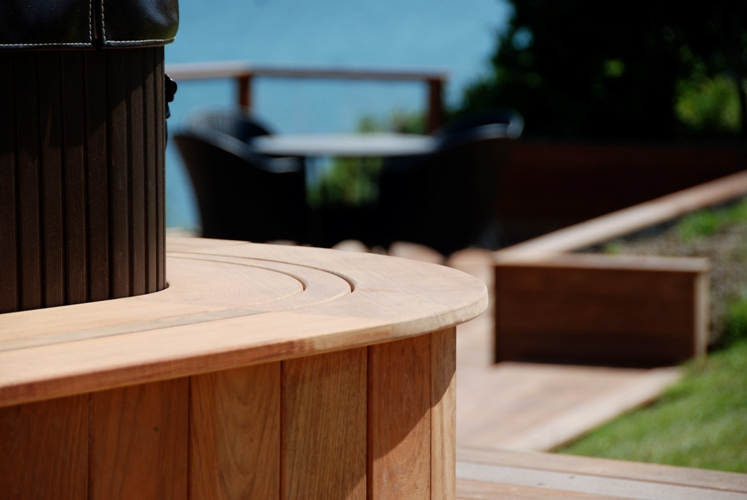
\includegraphics[width=\paperwidth,height=\paperheight,%
keepaspectratio]{Halvorsen.JPG}%
\vfill
}}}